\documentclass[11pt]{article}
\usepackage{color}
\usepackage{authblk}%allows footnote format for authors
\usepackage[letterpaper, margin=1in]{geometry} %package that allows changes in margins and header/footers
\usepackage[numbers,sort]{natbib}
\usepackage{amsmath}
\usepackage{rotating}
\usepackage{adjustbox}
\usepackage[english]{babel}
\usepackage{colortbl}
\usepackage{booktabs}
\usepackage[x11names,dvipsnames,table]{xcolor}
\bibliographystyle{ieeetr}
\newcommand{\mbh}[1]{\textcolor{orange}{ \emph{\scriptsize  #1}} } %creating command for Matt's comments
\newcommand{\lwang}[1]{\textcolor{red}{ \emph{\scriptsize  #1}} } %creating command for Li's comments
\newcommand{\gmj}[1]{\textcolor{blue}{ \emph{\scriptsize  #1}} } %creating command for Garrett's comments

\title{Review: Adaptive Introgression Expanded the Genetic Base of Crops during post-Domestication Spread}

\author[1]{Authors: Garrett M. Janzen}%author information
\author[1]{Li Wang}
\author[1,*]{Matthew B. Hufford}
\affil[1]{Department of Ecology, Evolution, and Organismal Biology, Iowa State University, Ames, Iowa, USA}
\affil[*]{Correspondence: mhufford@iastate.edu (M.B. Hufford)}
\date{}

\begin{document}



\maketitle

%Short Research reviews should be in the range 3500–4000 words, with up to 40 references and 6 figures/tables.


The process of domestication is often conceptualized as geographically constrained, with crops originating from a wild progenitor within one or more defined centers followed by expansion to the modern-day extent of cultivation \cite{Harlan1992}.
However, archaeological and genetic evidence are beginning to reveal that, in many cases, domestication has been temporally protracted and geographically diffuse \cite{brown2009complex, Meyer2016, wang2017, zhou2017, Fuller2014}.
An additional important aspect of the emerging complexity of domestication is beneficial gene flow (\emph{i.e.}, adaptive introgression) from locally adapted wild relatives during crop expansion following initial domestication.


Adaptive introgression has three components: hybridization between two genomes, backcrossing to one of the parents, and selection on different recombinant genotypes with progressively diminished linkage drag \cite{barton2001role, Feuillet200824}.
In domesticated species, adaptive introgression would consist of crop/wild hybrids backcrossing to a crop, retention and increase in frequency of adaptive wild haplotypes in the crop, and selection against undesirable wild background.
To date, literature on crop-wild gene flow has focused on the risk of transgene introgression from domesticated crops into wild relatives (for a review, \cite{stewart2003transgene}) and on modern plant breeding efforts to introgress desired traits from wild relatives (for a review, \cite{Dempewolf2017}).
The history of natural introgression of wild alleles into domesticated crops over evolutionary timescales has received considerably less attention.
However, new tools and methods have recently been employed to detect genome-wide patterns of introgression, granting new insights into the prevalence of adaptive introgression in crop histories.
Preliminary results suggest a need to expand our conception of domestication to include the broadening of the genetic base of crops that occurred during post-domestication expansion through gene flow with newly encountered wild relatives.


In this review, we will: 1) briefly describe recently developed methods for detecting adaptive introgression and provide a summary of how they can be applied to detect crop-wild introgression, 2) present case studies suggesting wild-to-crop introgression has conferred local adaptation, 3) consider how introgression bears upon fundamental questions of domestication, and 4) describe future advances in both basic and applied genetics that can be made through the study of introgression in agroecosystems.


\section*{Introgression methods and their application}

\mbh{In this section, I think the overall content is good, but we need to edit to make it more accessible and more explicit about how methods are implemented to detect adaptive introgression}

The decreasing cost of genome-wide resequencing and availability of reduced-representation genotyping (\emph{e.g.}, GBS and RAD-Seq), combined with new analytical methods, has facilitated comprehensive study of introgression across a number of species (\textbf{Table 1}).
High-density marker data can be used with haplotype-based and other methods to assign specific genomic regions to a taxon of origin and identify introgression across taxa \cite{Martin2015,Price2009,Lawson2012,pease2015,rosenzweig2016,geneva2015}.
The methods reviewed here do not include those marginally estimating introgression\slash migration rate as a component of demographic history (\emph{e.g.}, Approximate Bayesian Computation (ABC) \cite{beaumont2002}, diffusion approximations for demographic inference ($\delta a\delta i$) \cite{gutenkunst2009}, isolation with migration models \cite{hey2004}, and a series of methods utilizing the sequentially Markovian coalescent (PSMC, MSMC and SMC++) \cite{li2011, schiffels2014, terhorst2017}). 
Rather, we focus on methods that explicitly identify introgressed genomic segments based on the extent of differentiation, on patterns of nucleotide/haplotype sharing, and phylogenetic relationships.
%We focus here on analytical prospects and limitations and introduce only a few representatives of each category.

First, introgressed segments are expected to show low differentiation from their source population.
The $F_{st}$ and $d_{XY}$ statistics and their derivates including $G_{min}$ \cite{geneva2015} and $RND_{min}$\cite{rosenzweig2016} gauge differentiation. 
The former two statistics are insensitive to rare migrants and therefore lack power to detect recent introgression, while the latter two overcome this limitation.
Additionally, $RND_{min}$ accounts for variable mutation rate, which is detected based on branch length to an outgroup: 

% \begin{equation}
%    G_{min} = \frac{d_{min}}{d_{XY}}
% \end{equation}
% where $d_{min}$ is the minimum sequence distance between haplotypes in species X and Y.
 
 \begin{equation}
 	RND_{min} = \frac{d_{min}}{d_{out}}
 \end{equation}
where $d_{min}$ is the minimum sequence distance between haplotypes in species X and Y and $d_{out}$ equals $(d_{XO} + d_{YO})/2$, the average sequence distance between each species and the outgroup ($O$).
 
These statistics have recently been further developed by adding differentiation between both non-admixed ($A$) and admixed populations ($B$) and a source population ($C$) \cite{racimo2016}. 
For example, the $U_{A,B,C(w,x,y)}$ statistic summarizes number of sites where an allele at frequency $y$ in the source population ($C$) has a frequency higher than $x$ in the admixed population ($B$) and lower than $w$ in the non-admixed population ($C$).
A similar statistic, $Q95_{A,B,C(w,y)}$, sets a hard cutoff at the $95^{th}$ percentile of allele frequencies in the admixed population (B) \cite{racimo2016}.
Further modifications have allowed specification of more than one source population (see details in \cite{racimo2016}).
 
Second, local ancestry deconvolution (also known as chromosome painting) assigns genomic regions to various source populations based on patterns of allele/haplotype sharing \cite{schraiber2015}. 
One form of chromosome painting utilizes hidden Markov models to evaluate ancestry across admixed genomes through comparison to reference, non-admixed individuals (\emph{e.g.}, HAPMIX \cite{Price2009}). 
Another clusters admixed populations with reference samples using a sliding-window approach (\emph{e.g.}, PCAdmix \cite{brisbin2012pcadmix} and LAMP \cite{sankararaman2008}).
And finally, introgression can be detected through chromosome painting by using a Bayesian model \cite{pritchard2000} in which deviations from Hardy-Weinberg equilibrium are minimized through creation of genetic groups (\emph{e.g.}, fineSTRUCTURE \cite{Lawson2012}). 

\gmj{Li, are you familiar with the analytical tools MIGRATE-N and BAYESASS?  Rieseberg comapres these two to STRUCTURE at some length in the discussion of this paper:
https://biology.unm.edu/Whitney/Whitney%20Reprints/Scascitelli%20et%20al%202010.pdf
Should we include these two methods, even in passing, in this portion of the paper?}
\lwang{Garrett, I donot know these two methods. I am reading the paper you mentioned here.}

Third, the ABBA-BABA statistic (also known as the D-statistic) and its derivatives are widely applied to introgression detection.
These statistics make inferences regarding introgression based on genomic patterns of derived variants that are shared between populations or species.
Patterns of allele sharing are interpreted in a phylogenetic context and the method is best suited to detection of introgression at the genome level.
Elaborations of the D-statistic capable of localizing introgression to specific genomic regions include $\hat{f_{d}}$ \cite{Martin2015} and the five-taxon D-statistic \cite{pease2015}. 
The former is quite similar to the D-statistic but uses allele frequencies from each population/species, and the latter detects introgression based on the localized phylogenetic pattern and is capable of determining introgression directionality.

Application of these approaches across a number of plant and animal species suggests introgression can play an adaptive role. For example, introgression from ancient hominins (\emph{e.g.}, Neanderthals and Denisovans) to humans has been detected at loci controlling skin pigmentation, defense against pathogens, and toleration of high altitude (reviewed in \cite{Racimo2015}); introgression has conferred M\"{u}llerian mimicry \mbh{I would explain a bit more here...wing coloration loci, protects against predation...} across butterfly species \cite{Heliconius2012}; introgression has spread insecticide resistance across mosquito species \cite{Norris2015}, and introgression across \emph{Mimulus} (\emph{i.e.}, monkeyflower) species has resulted in adaptation to pollinator preference and contributed to speciation \cite{Stankowski2015}.






\section*{Crop adaptation through introgression}

Genome-wide data from extensive samples of crops and their wild relatives, in combination with the new methods described above, have recently allowed detailed analysis of wild-to-crop introgression in some of the world's most important crops (\textbf{Table 2}).
Below we present a summary of findings from maize, barley, and rice, three promising systems in which introgression from wild relatives may have played an adaptive role.

\begin{enumerate}
\item{Maize:}


The relationship between maize (\emph{Zea mays} ssp. \emph{mays}) and the teosinte \emph{Zea mays} ssp. \emph{mexicana} (hereafter, \emph{mexicana}) offers a prime case study of adaptive wild-to-crop introgression.
Maize was domesticated from \emph{Zea mays} ssp. \emph{parviglumis} (hereafter, \emph{parviglumis})  approximately 9,000 years ago in the lowlands of the Balsas River Valley in Mexico \cite{matsuoka2002single}.
From this domestication center, maize spread into the highlands of the Mexican Central Plateau, where it came into sympatry with \emph{mexicana}.
Introgression from \emph{mexicana} to maize in the Central Plateau has been reported based on both morphological \cite {wilkes1977} and molecular \cite{vanHeerwaarden2011, doebley1987} data.
However, \citep{hufford2013} first localized \emph{mexicana} introgression to chromosomal regions and provided evidence that it was likely adaptive.
%The following is not fully clear.  Cut or revise.
The authors identified nine genomic regions in several maize populations which consistently showed evidence of \emph{mexicana} introgression based on chromosome painting using both HAPMIX and the linkage model of STRUCTURE (Figure \ref{fig:introgressionMaize}).
These introgressed segments overlapped QTL that had previously been found to control anthocyanin content and leaf macrohairs \cite{lauter2004}, traits known to be adaptive at high elevation.
In a growth chamber experiment, the authors demonstrated that maize populations with \emph{mexicana} introgression showed greater plant height (a proxy for fitness) under highland environmental conditions than populations that lacked introgression.
Height differences were not detected under lowland conditions.
%Among the nine regions, three span the centromeres of chromosomes 5, 6, and 10, and one is located in the inversion polymorphism on chromosome 4, suggesting a significant role of genome structures restricting recombination in adaptive introgression.
%In summary, the introgressed alleles/haplotypes from \emph{mexicana} to maize conferred adaptation to highland habitats when maize migrated from Mexican lowlands.


%Even though introgression from \emph{mexicana} to Mexican highland maize has been highly supported, it is yet unknown whether and to what extent such introgression could be found in other highland maize populations which are allopatric to \emph{mexicana}. 
%A recent study \cite{Takuno2015} found little empirical or theoretical support for parallel highland adaptation in the Mexican and South American highland regions, which was explained partly by the difference in potential for adaptive introgression from wild relatives.
%Adaptive SNPs in Mexican highland population were more likely located in the introgressed regions than those in South American highland populations.
%Furthermore, the adaptive SNPs in the Mexican highland population were more likely also showing signatures of local adaptation in \emph{mexicana} and \emph {pulviglumis} populations than those South American highland population.
%For these reasons, adaptive introgression from wild relatives may play a significant role in patterning the genetic differences of maize highland populations.

Populations of \emph{mexicana} cannot be found outside of the highlands of Mexico, yet maize has colonized and adapted to high elevation in a number of other regions.
%Several questions regarding \emph{mexicana} introgression yet remain.
%Has the introgression from \emph{mexicana} spread to multiple highland populations? 
%How do highland-adaptation traits differ among populations with and without introgression from \emph{mexicana}?
A recent study \cite{wang2017} employed the ABBA-BABA and $\hat{f_{d}}$ statistics to evaluate whether maize with \emph{mexicana} introgression was transferred to other highland regions or whether highland adaptation was obtained \emph{de novo} outside of Mexico.
%On chromosome 4 (Figure \ref{fig:fd}), Mexican highland (MexHigh) and Guatamalan highland (GuaHigh) exhibited strong evidence of introgression from \emph{mexicana}, and the peaks of distribution corresponded to the region identified in Hufford et al. (2013) \citep{hufford2013}.
%The signal of introgression is absent for the other three populations.
%On chromosome 5, the signals of introgression (the peak region of the distribution) are present in MexHigh, GuaHigh and Southwestern US Highland (SW\_US), but not the other two.
%More details on the other chromosomes can be found in \cite{Wang2015manuscript}.
Overall, analyses revealed that maize landraces with \emph{mexicana} introgression were transferred to nearby high elevation regions in Guatemala and the southwestern United States, but more distant high elevation regions (\emph{e.g.,} the Andes) showed no \emph{mexicana} ancestry. 
%The Andean maize, the population totally isolated from the occurrence of any teosinte species, underwent the severest historical bottleneck, as a population in the front wave of the serial founder effects. 
%The stronger genetic drift introduced by the smaller historical population size increased homozygosity but reduced the heterozygosity of the population, and it also extended the length of homozygosity.
%The high frequency of deleterious alleles caused by stronger genetic drift in the Andes population, together with the reduced efficiency of selection against deleterious sites, contributes to the observed higher mutation load in the well-isolated maize population.
%Although it is clear that the absence of introgression from wild relatives provided fewer genetic resources for highland adaptation (making the highland adaptation in the Andes unique), it is yet unknown whether or not being out of reach of wild relatives is a reason for reduced fitness in the Andes population.
%Furthermore, the question of whether convergent evolution occurs between populations with and without introgression from wild relatives is a key topic for future studies in maize.
Historically, \emph{mexicana} haplotypes appear to have played an important role in adaptation of maize to challenging high-elevation conditions.
Breeding programs for highland maize may further benefit from drawing on \emph{mexicana} germplasm, particularly in regions like the Andes where \emph{mexicana} alleles are not known to have spread.


\begin{figure}[h]
	\centering
	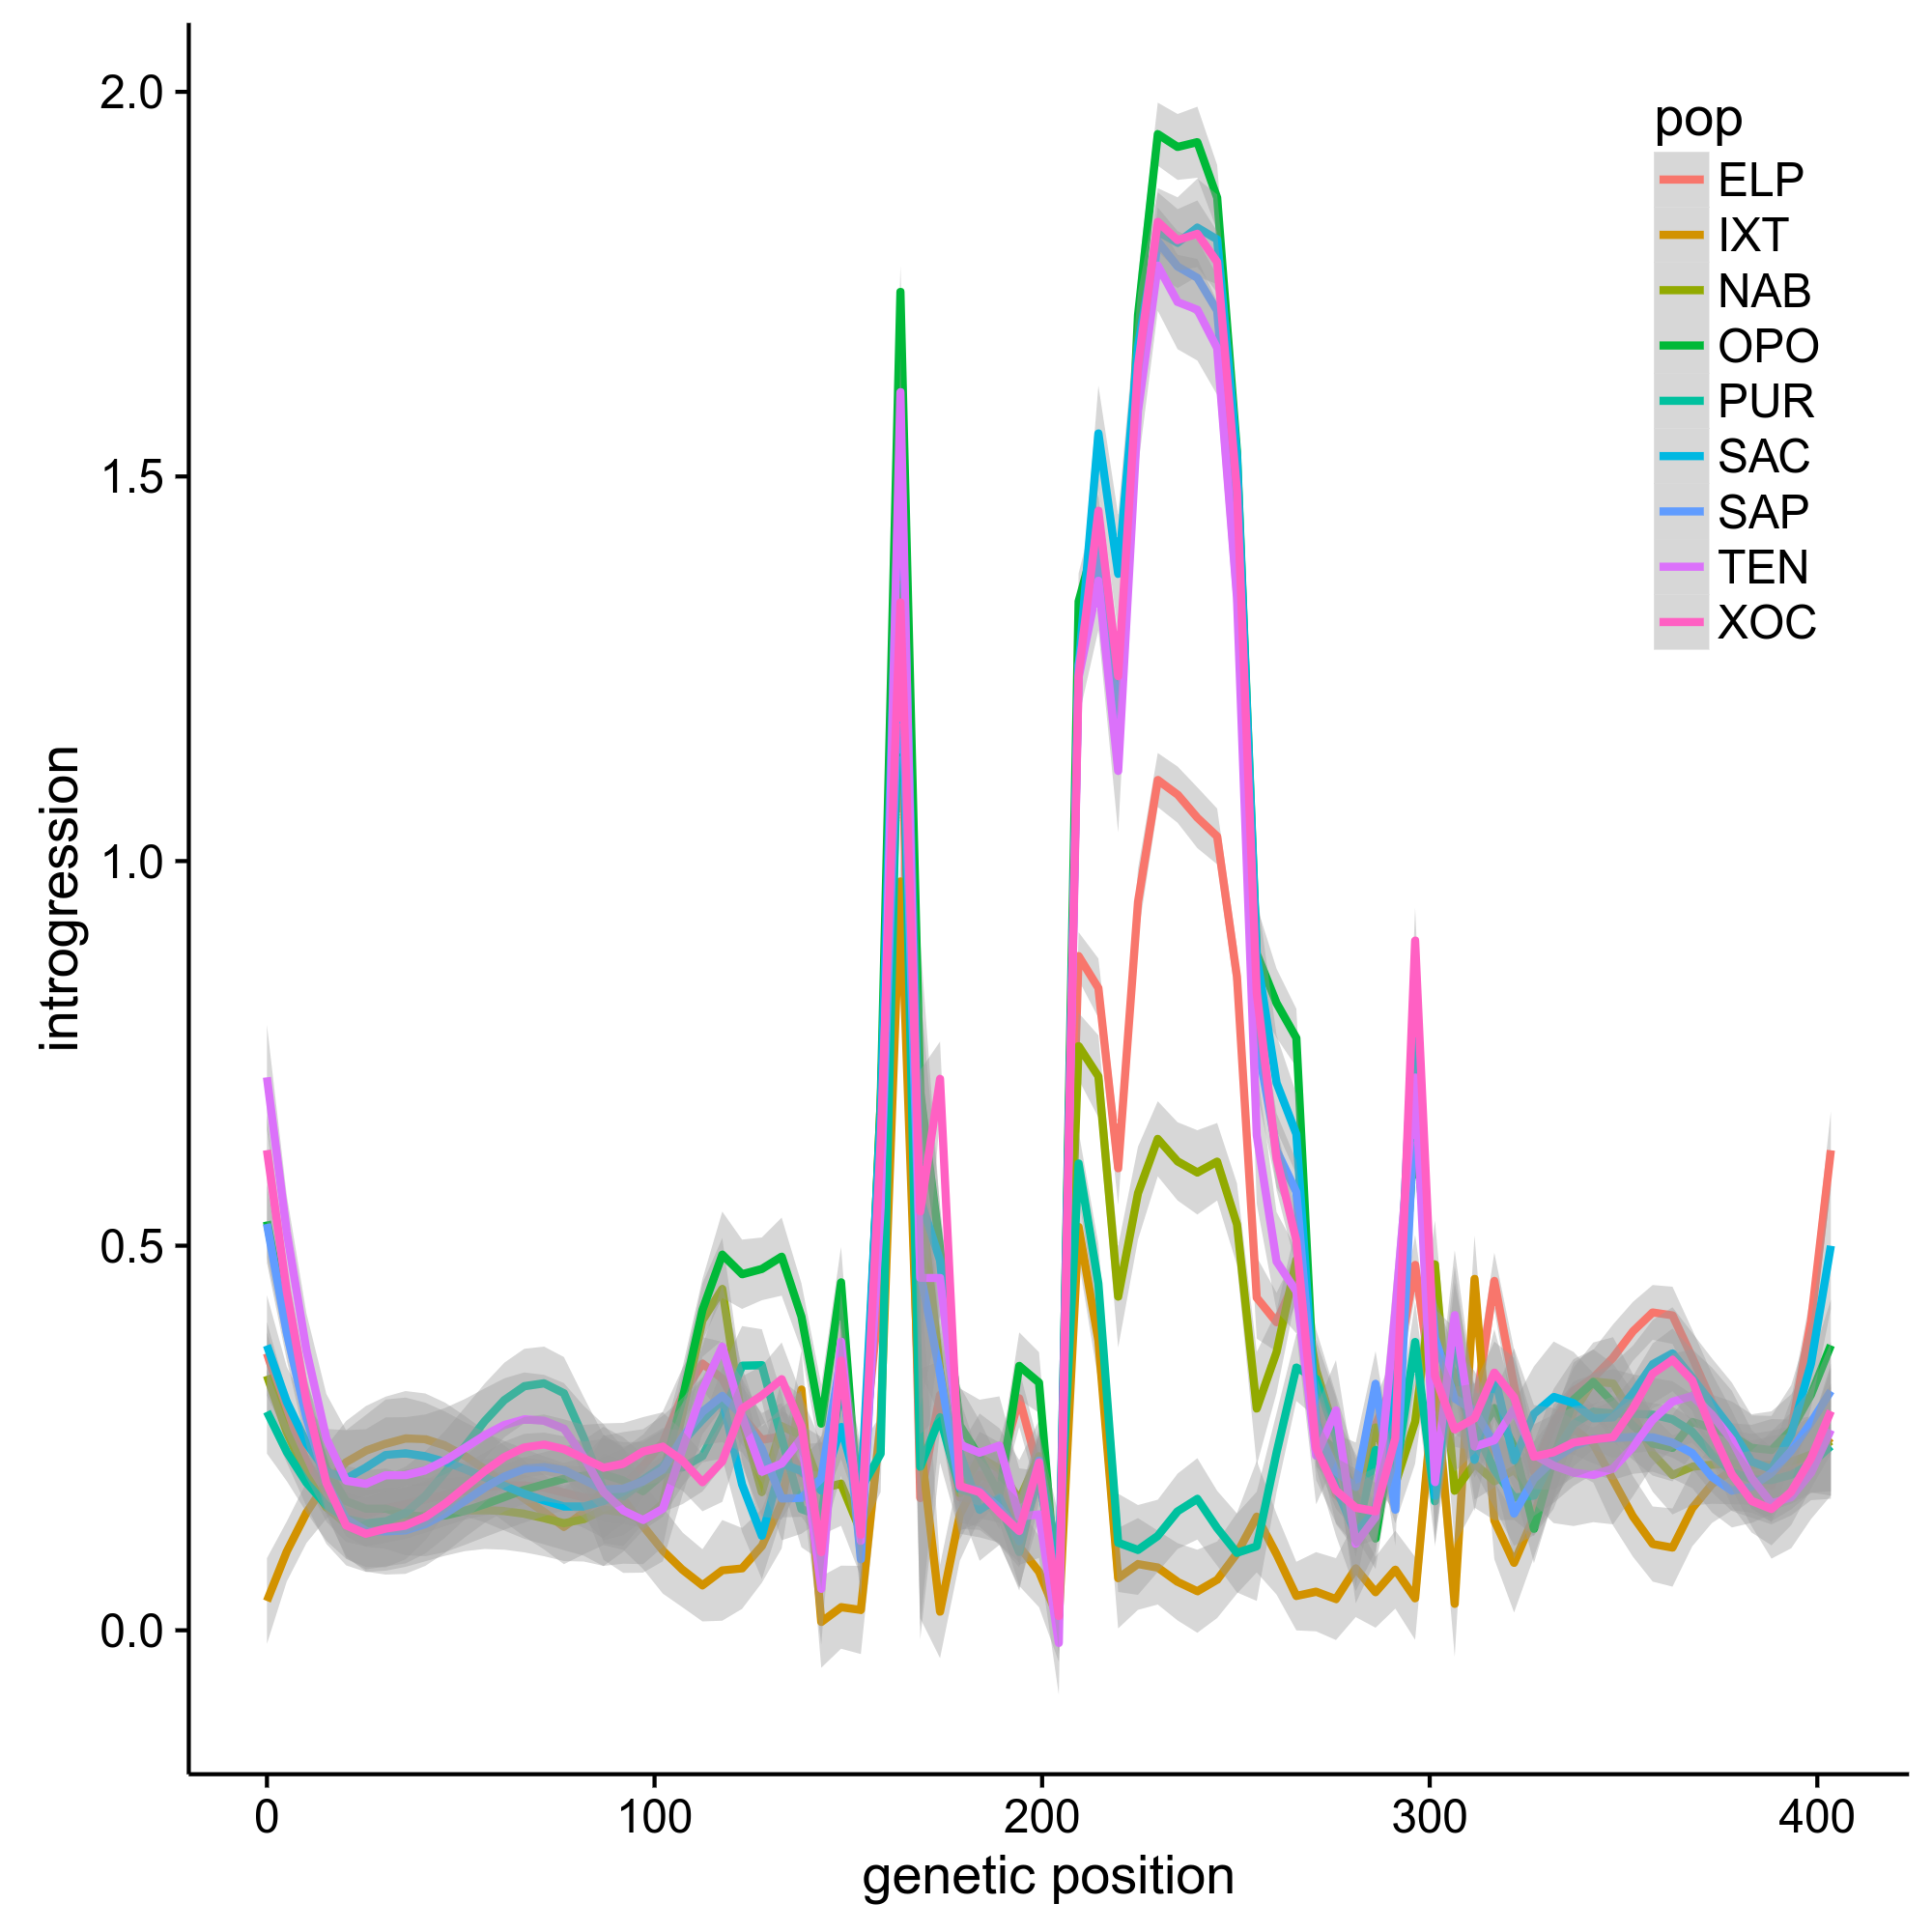
\includegraphics[width=17.35cm]{li_figure.png}
	\caption{Li's caption here.}
	\label{fig:introgressionMaize}
\end{figure}













\item{Barley:}
		
%Domesticated and wild barley belong to the same species, \emph{Hordeum vulgare}, and are capable of producing viable offpspring via hybridization \cite{von1995ecographical}.
Barley (\emph{Hordeum vulgare} subsp. \emph{vulgare}) was domesticated at least twice roughly 8,000 to 10,000 BP: once from the wild subsp. \emph{spontaneum} in the Fertile Crescent and once from subsp. \emph{spontaneum} var. \emph{agriocrithon} in Tibet \cite{takahashi1955origin, badr2000origin, azhaguvel2007phylogenetic, haberer2015barley, ren2013tibet, dai2012tibet}.
%\gmj{While morrell2007 cites the Zargos mountains as a center of domestication, this paper is cited by ren2013tibet, which states that the findings of morrell2007genetic are just that a second origin exists east of the Fertile Crescent. It is cited by dai2012tibet and the poets paper, but little is said of its mention of the zargos mountains.  I think that the mention of the Zargos mountains was just as a dividing line between the two spheres of influence between the two domestication centers.}
Presently, the distribution of subsp \emph{spontaneum} stretches from the eastern Mediterranean through the Middle-East to west-central Asia spanning clines in temperature, precipitation, soil type, and altitude \cite{nevo2010drought}.
Barley/\emph{spontaneum} hybrids are fertile and found spontaneously when wild and domesticated barley co-occur.
Introgression between wild and domesticated barley is frequent \cite{dai2012tibet}, at times occurring over distances greater than a kilometer \cite{hillman2001new}.

%The barley domestication process has reduced the number of alleles in the domesticate to only 40\% of that found in wild barley, though there remains a great deal of phenotypic diversity among the wild barleys \cite{ellis2000wild}.

Poets and co-authors \cite{Poets2015} investigated the range-wide contribution of wild barley to landraces, assessing both genome-wide and geographical patterns.
This study identified several lines of evidence consistent with wild introgression aiding the dispersal and adaptation of domesticated barley.
Genomic regions of shared ancestry were detected linking individual landraces to a number of wild relative populations, suggesting landraces may have received wild introgression on a continual basis during post-domestication expansion.
However, barley landraces showed an excess of ancestry from nearby wild relatives, indicating a prevalence of local and potentially adaptive gene flow.
Low linkage disequilibrium and small blocks of identity by state indicated even these locally introgressed regions are old, perhaps dating back to the early expansion of barley following domestication.
While these results are suggestive, wild barley haplotypes have yet to be definitely linked to specific local adaptations in landraces.

%Genomic evidence points to a history of wild-to-crop introgression during dispersal of barley beyond their centers of domestication, but for the most part, the identity of the alleles critical to these adaptations have yet to be uncovered.
%One exception comes from the authors of \cite{dai2012tibet}, who hypothesize that alleles for cold stress tolerance and spring habit \gmj{"spring habit" are the words from the paper, but they're not defined.  Does this mean that it grows more quickly in the spring?} from wild Tibetan 2-rowed barley allowed the barley to spread to the cold northern regions of Europe.
%Wild-domesticate breeding experiments have shown that wild barleys have alleles for several important fitness and agronomic phenotypes, including powdery mildew resistance, brittleness, flowering time, plant height, lodging, and yield \cite{dreiseitl2017heterogeneity,von2006ab,handley1994chromosome}, and these individually or in combination may have been facilitators of the dispersal of domesticated barley.












\item{Asian Rice:}

The story of Asian rice (\emph{Oryza sativa}) domestication is still debated, with hybridization between wild and domesticated rice contributing to the complexity of this crop's history.
On one hand, some genetic and archaeobotanical evidence point toward independent domestications of the two prominent varietal groups \emph{japonica} and \emph{indica} from the wild species \emph{Oryza rufipogon} (\emph{rufipogon} hereafter) in the Yangtze Basin and the Indian Ganges plain, respectively \cite{fuller2010consilience}.
Other studies support a single domestication occurring 8,200-13,500 BP in the Yangtze Basin in China from \emph{rufipogon}, with later divergence of \emph{indica} and \emph{japonica} \cite{molina2011molecular}.
Huang and colleagues \cite{Huang2012} developed a genetic map of rice variation, which they used to measure genetic distance between wild and domesticated rices at and around domesication loci for various geographical locations, finding that \emph{japonica} was likely domesticated in the Pearl River area of Guangxi province, China (just south of the Yangtze Basin), and that \emph{indica} was likely the result of hybridization between \emph{japonica} and local \emph{rufipogon} populations in Southern and South-eastern Asia. %Also, Huang includes the following quote: "We noticed that many loci with strong signals of selection were nearly identical in both indica and japonica where FST between indica and japonica was extremely low, indicating that introduction of traits during domestication has in many cases involved introgression events."


%The former first paragraph, replaced from above:
%The story of Asian rice (\emph{Oryza sativa}) domestication is still debated.
%Interspecific hybridization between wild and domesticated rices both ancient and recent has produced a phylogeny that defies clear and simple models.
%On one hand, some genetic and archaeobotanical evidence point toward independent domestications of the two prominent varietal groups \emph{japonica} and \emph{indica} from the wild species \emph{Oryza rufipogon} (\emph{rufipogon} hereafter) in the Yangtze Basin and the Indian Ganges plain, respectively \cite{fuller2010consilience}.
%Other studies support a single center of domestication, arguing that present-day patterns of rice variation could be explained by a single domestication event in a population with high standing variation, followed by dispersal into sympatry with locally-adapted wild relatives in diverse environments, genetic admixture, and selection for adaptive alleles \cite{vaughan2008evolving}.
%A recent investigation utilizing SNP data from wild and domesticated rice accesssions pointed to a single domestication occurring 8,200-13,500 BP in the Yangtze Basin in China from rufipogon, with later divergence of \emph{indica} and \emph{japonica} \cite{molina2011molecular}.
%Huang and colleagues \cite{Huang2012} developed a genetic map of rice variation, which they used to measure genetic distance between wild and domesticated rices at and around domesication loci for various geographical locations, finding that \emph{japonica} was likely domesticated in the Pearl River area of Guangxi province, China (just south of the Yangtze Basin), and that \emph{indica} was likely the result of hybridization between \emph{japonica} and local \emph{rufipogon} populations in Southern and South-eastern Asia. %Also, Huang includes the following quote: "We noticed that many loci with strong signals of selection were nearly identical in both indica and japonica where FST between indica and japonica was extremely low, indicating that introduction of traits during domestication has in many cases involved introgression events."

%The former first paragraph, replaced from above:
%The story of Asian rice (\emph{Oryza sativa}) domestication is still debated.
%A recent investigation pointed to a single domestication occurring 8,200-13,500 BP in the Yangtze Basin in China from the wild species \emph{Oryza rufipogon} (\emph{rufipogon} hereafter), with later divergence of the two prominent varietal groups, \emph{japonica} and \emph{indica} \cite{molina2011molecular}.
%\cite{vaughan2008evolving} support this view, noting that present-day patterns of rice variation could be explained by a single domestication event in a population with high standing variation, followed by dispersal into sympatry with locally-adapted wild relatives in diverse environments, genetic admixture, and selection for adaptive alleles.
%On the other hand, genetic and archaeobotanical evidence point toward independent domestications of \emph{japonica} and \emph{indica} in the Yangtze Basin and the Indian Ganges plain, respectively \cite{fuller2010consilience}.
%An alternative explanation, as described by \cite{Huang2012}, suggests an initial domestication of \emph{japonica} in China followed by formation of the \emph{indica} group through hybridization of \emph{japonica} and local \emph{rufipogon} populations in Southern and South-eastern Asia.
%Adaptive introgression may in fact be the signal interpreted as independent domestications.

Vaughan and colleagues \cite{vaughan2008evolving} posit a hypothesis combining elements of both theories.
According to this hypothesis, the non-shattering allele arose in a single cultivated rice population and then introgressed into many diverse cultivated populations (some japonica-like, some indica-like) in the region.
This would have facilitated the subsequent spread of other domestication alleles among those populations.
As these domesticated populations then spread into new environments, they would have recieved introgressions from locally-adapted wild relatives, retaining alleles that improved fitness (in agreement with \cite{second1982origin}).
Contemporary populations of wild and domesticated rice show evidence of this history of local adaptation.
The wild relatives \emph{rufipogon} and \emph{nivara} both maintain high genotypic and phenotypic diversity and exhibit locally-adaptive traits (\emph{rufipogon} is adapted to forested wetland environments, whereas \emph{nivara} is adapted to dryer conditions and has life cycle adaptations to survive grazing pressure), suggesting that either offered (and offers) adaptive genetic potential.
Likewise, domesticated rice varieties display patterns of local adaptation (for examples, two of the domesticated rice deepwater varieties (\emph{rayada} and \emph{ashwina}) are said to be selected for the environment along the Ganges river, the \emph{japonicas} are split into temperate and tropical subgroups, and the \emph{indicas} are best suited for lowland environments.

%Other studies support a single center of domestication, arguing that present-day patterns of rice variation could be explained by a single domestication event in a population with high standing variation, followed by dispersal into sympatry with locally-adapted wild relatives in diverse environments, genetic admixture, and selection for adaptive alleles \cite{vaughan2008evolving}.
%The high genetic diversity within domesticated rice is likely due to introgression from wild relatives both within the domestication center(s) and in new environments where rice has dispersed \cite{second1982origin}, and gene flow between domesticated Asian rice and its wild relatives outside of the Yangtze Basin could have imparted locally adaptive traits \cite{vaughan2008evolving}.
%The wild relatives \emph{rufipogon} and \emph{nivara} both maintain high genotypic and phenotypic diversity and exhibit locally-adaptive traits (whereas \emph{rufipogon} is adapted to forested wetland environments, \emph{nivara} is adapted to dryer conditions and has life cycle adaptations to survive grazing pressure).
%From Huang2012, "Based on the SNP data, the sequence diversity (p) of O. rufipogon was estimated at 0.003, which is higher than that in O. sativa—the sequence diversity is 0.0024 for O. sativa, and 0.0016 and 0.0006 for indica and japonica, respectively21".
%Likewise, domesticated rice varieties display patterns of local adaptation (for examples, two of the domesticated rice deepwater varieties (\emph{rayada} and \emph{ashwina}) are said to be selected for the environment along the Ganges river, the \emph{japonicas} are split into temperate and tropical subgroups, and the \emph{indicas} are best suited for lowland environments.
%Gene flow between wild and cultivated rices, though asymmetrical, is frequent enough that nuisance weedy hybrids commonly arise amongst cultivated populations and must be managed with difficulty \cite{vaughan2008evolving}.

To date, research into adaptive introgression in the domestication of rice has been insufficient to detect clearly-supported examples (though \cite{zhao2010genomic} emphasizes the necessity of this research).
%\cite{zhao2010genomic} used a SNP panel and STRUCTURE analysis to uncover patterns of population structure, admixture, and introgression within domesticated rices, and the authors emphasize the importance of similar research that includes wild rice accessions.
There are perhaps some practical reasons why research has not yet been devoted to this inquiry.
As with many other domesticated crops, gene flow between wild and domesticated rices is highly asymmetric (estimates of wild rice admixture in domesticated rice are less than 5 percent \cite{wang2017asian}).
This asymmetry is due in part to the closed floret architecture of the domesticated rice, which hinders outcrossing.
Crop-wild ybridization is frequent enough that nuisance weedy hybrids commonly arise amongst cultivated populations and must be managed with difficulty \cite{vaughan2008evolving}.
During early domestication, introgression may have been more prevalent than at present because barriers to crop-to-wild introgression may have been less severe and because the inbreeding reproductive system of rice would not have been as firmly established \cite{vaughan2008evolving}.
Furthermore, the contemporary distribution of wild rice does not capture the range and diversity of wild rice during early domestication and range expansion of rice.

%Introgression into indica is expected to be more likely than japonica, due to the higher degree of sympatry between indica and its wild relatives.

%note from Asian wild rice is a hybrid swarm with extensive gene flow and feralization from domesticated rice:
%Cite this paper to talk about how the ranges of the several subspecies of domesticated rice are distinct/sometimes overlap.  The paper makes the point that this overlap helps facilitate gene flow.








\end{enumerate}

	

	
	
	
	
	
	
	
	



\begin{table}
\rowcolors{2}{white}{gray!25}
\begin{center}
\caption{List and brief description of recently developed methods and examples of empirical studies employing these methods.} \label{tab:tools}
\begin{tabular}{llll}
\\\toprule  
\rowcolor{white}
{\bf methods}	& {\bf data type } &	{\bf reference} &  {\bf empirical studies } \\ \midrule

\rowcolor{gray!25}
{\emph{\bf chromosome paiting}} &   &   &   \\
\rowcolor{gray!25}
Hapmix	& phased haplotype; reference panel		& Price et al. 2009	&  Hufford et al. 2013;  Suarez et al. 2016 \\ 
\rowcolor{gray!25}
RASPberry &	phased haplotype &	Wegmann et al. 2011	 & Christe et al. 2016 \\
\rowcolor{gray!25}
MultiMix & phased/unphased genotype; reference panel &	Churchhouse and Marchini 2013 &	Eyheramendy et al. 2015 \\
\rowcolor{gray!25}
PCAdmix	 & phased haplotype	 & Brisbin et al. 2012	 & Moreno et al. 2014; Pugach et al. 2016 \\
\rowcolor{gray!25}
LAMP  &	phased haplotypes; reference panel	 & Sankararaman et al. 2008	 & Patterson et al. 2012 \\

\rowcolor{white}
{\emph{\bf phylogenetic relationship}} &   &   &   \\
\rowcolor{white}
ABBA-BABA/D-statistics	 & biallelic SNP  &	Durand et al. 2011	 &  Heliconius Genome Consortium 2012 \\
\rowcolor{white}
fd statistic &	biallelic SNP &	Martin et al. 2015  &	Malinsky et al. 2015; Zhang et al. 2016 \\ 
\rowcolor{white}
five taxon D statistics	& biallelic SNP	&  Pease and Hahn 2015	& Fontaine et al. 2015; Pease et al. 2016 \\

\rowcolor{gray!25}
{\emph{\bf divergence}} &   &   &   \\
\rowcolor{gray!25}
Gmin &	biallelic SNP	&  Geneva et al. 2015	&  Kingan et al. 2015 \\
\rowcolor{gray!25}
RNDmin	& phased haplotype	& Rosenzweig et al. 2016	&  NA \\
\rowcolor{gray!25}
(see .tex file for comment) & biallelic SNP & Racimo et al. 2016 & Sams et al. 2016 \\

%I was not able to add Li's entry to this cell without errors.  I'll put her entry in the line below:
%U_{A,B,C(w,x,y)} and Q95_{A,B,C(w,y)}

\end{tabular}
\end{center}
\end{table} 

\begin{table}
\centering
\begin{adjustbox}{width=1\textwidth}
\small
\label{my-label}
\begin{tabular}{|p{5cm}|p{5cm}|p{2.6cm}|p{2.6cm}|p{2.6cm}|l|}
\hline
Crop & Compatible Wild Relatives & Hybrids and/or Hybridization & Evidence of Crop Introgression & Evidence of Adaptiveness & Source \\ \hline \hline
Maize (\emph{Zea mays} subsp. \emph{mays}) & \emph{Z. m.} subsp. \emph{mexicana}, \emph{Z. m. } subsp. \emph{parviglumis} & X & X & X & \cite{hufford2013genomic} \\ 
\hline 
Asian Rice (\emph{Oryza sativa}) & \emph{O. rufipogon} & X & X & X & \cite{Huang2012} \\ 
\hline
Barley (\emph{Hordeum vulgare}) & \emph{H. v.} subsp. \emph{spontaneum} & X & X & X & \cite{Poets2015} \\ \hline
Sunflower (\emph{Helianthus annuus}) & \emph{H. argophyllus}, \emph{H. bolanderi}, \emph{H. debilis}, \emph{H. petiolaris} & X &   &   & \cite{rieseberg2007hybridization}\\ 
\hline
Cassava (\emph{Manihot esculenta}) & \emph{M. glaziovii} & X & X & X & \cite{bredeson2016sequencing} \\ 
\hline
Potato (\emph{Solanum tuberosum}) & many & X & X & X & \cite{johns1986ongoing, gavrilenko2013genetic} \\
\hline
Tomato (\emph{Solanum lycopersicum}) & \emph{S. pimpinellifolium} & X & X & X & \cite{rick1958role} \\
\hline
Olive (\emph{Olea europaea} ssp. \emph{europaea} var. \emph{sativa}) & \emph{O. e.} ssp. \emph{europaea} var. \emph{sylvestris} & X & X & & \cite{diez2015olive} \\ 
\hline
Soybeans (\emph{Glycine max}) & \emph{G. soja} & X & X &  & \cite{lam2010resequencing} \\ 
\hline
Common Bean (\emph{Phaseolus vulgaris}) & \emph{P. v.} var. \emph{aborigineus, P. v.} var. \emph{mexicanus} [[not in this source]]& X & X &  & \cite{papa2003asymmetry} \\
\hline
Grapes (\emph{Vitis vinifera} subsp. \emph{vinifera}) & \emph{V. v.} subsp. \emph{sylvestris} & X & X &  &  \cite{myles2011genetic} \\
\hline
Sorghum (\emph{Sorghum bicolor} subsp. \emph{bicolor}) & \emph{S. b.} subsp. \emph{arundinaceum, S. b.} subsp. {drummondii} & X & X &  & \cite{aldrich1992patterns} \\
\hline
Wheat (\emph{Tritium monococcum, T. dicoccum, T. aestivum}) & \emph{T. m. boeoticum, T. dioccoides, T. urartu, Aegilops speltoides, A. tauschii} & X & X &  & \cite{zohary1969wild} \\
\hline
Apple (\emph{Malus domesticus}) & \emph{M. sylvestris}, \emph{M. orientalis}, \emph{M. baccata}, \emph{M. sieversii}  & X & X & & \cite{cornille2012new} \\
\hline
\end{tabular}
\end{adjustbox}
\end{table}

%\begin{figure}[h]
%	\centering
%	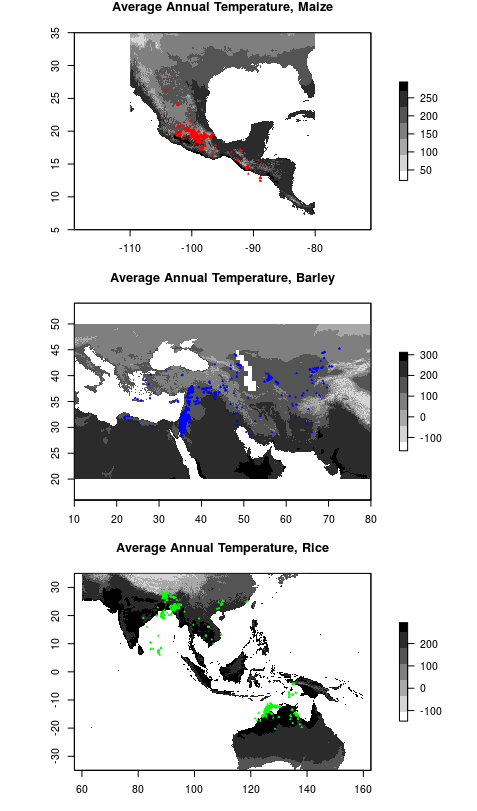
\includegraphics[width=17.35cm]{vertical.png}
%	\caption{Map of the natural ranges of wild relatives of four domesticated crops, overlayed with average annual temperature.}
%	\label{boxplot:map}
%\end{figure}

\begin{figure}[h]
	\centering
	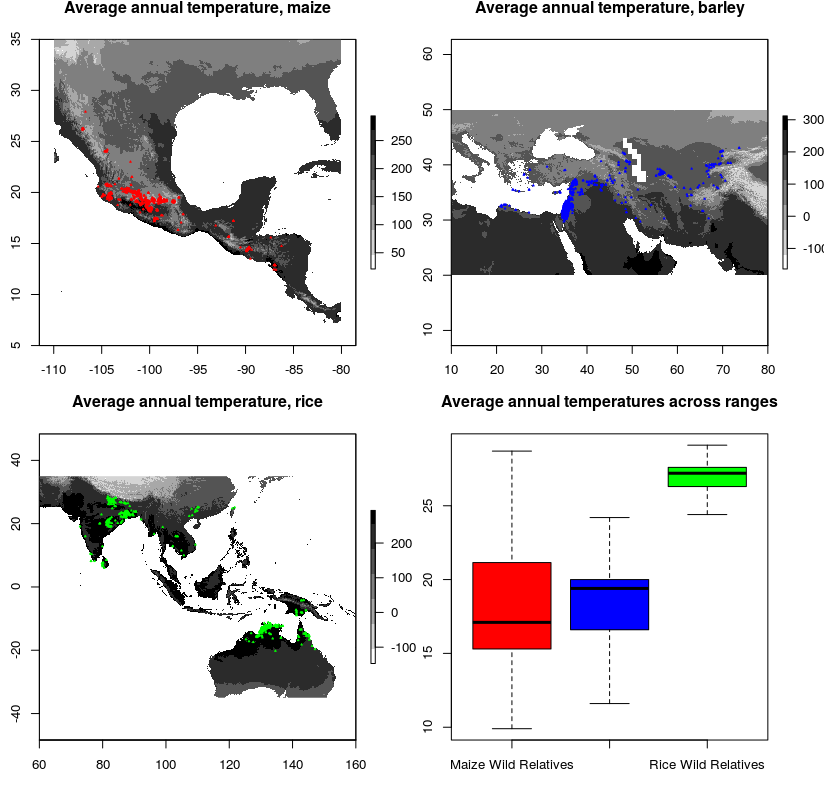
\includegraphics[width=17.35cm]{combination.png}
	\caption{Map of the natural ranges of wild relatives of three domesticated crops, overlayed with average annual temperature. The distribution of average annual temperature experienced in the geographic home ranges of wild relatives interfertile with four crops}
	\label{fig:map}
\end{figure}

\section*{Re-evaluating domestication}

A framework in which crops are domesticated from a single wild population or even a single species is an oversimplification when introgression during the geographic expansion of crops is extensive.
The addition of ongoing gene flow to our understanding of crop demography could bear importantly on fundamental questions of crop domestication:

\subsection*{What is the progenitor of a crop?}
Depending on the extent of post-domestication gene flow with new wild relatives, identification of a crop's progenitor can be complicated or completely confounded.
The level of divergence of a crop from newly encountered populations and species will decrease due to introgression, a signal that could be mistaken for origin rather than gene flow.
For example, when determining a single origin of maize from \emph{parviglumis}, Matsuoka and colleagues \cite{matsuoka2002single} identified a paradox: while \emph{parviglumis} is found exclusively in the lowlands of southwest Mexico, maize with allele frequencies most similar to \emph{parviglumis} was found in the highlands of the Mexican Central Plateau.
Several years later, van Heerwaarden \emph{et al.} \cite{vanHeerwaarden2011} resolved the paradox by determining that widespread introgression in the highlands from \emph{mexicana}, which is closely related to \emph{parviglumis}, has caused maize from this region to appear ancestral.
Similarly, extensive post-domestication adaptive introgression from  potato wild relatives long obscured this crop's origin.
Recent work has shown that, following the original domestication event of \emph{Solanum tuberosum} in the central Andes, potato received introgression from as many as four additional species during colonization of the highest elevations of the Andes and the lowlands of the Chilean coast \cite{Spooner2014, Gavrilenko2013}.
Beyond confounding detection of progenitor taxa, extensive introgression may necessitate a reevaluation of crop origins.
In cases like maize and potato it is important to recognize the substantial contributions of introgressing taxa to the genetic base of modern crops.
Broad recognition of the role these wild relatives have played in crop adaptation could further their use in breeding and elevate their conservation status.

\subsection*{When was a crop domesticated?}
Estimates of the timing of initial domestication are often based on levels of sequence divergence between a crop and populations of its presumed progenitor (\emph{e.g.}, \cite{matsuoka2002single, molina2011molecular}).
In highly introgressed domesticates, these estimates will be based on comparison of either crop or introgressant haplotypes to those of the progenitor.
In such cases, divergence is a mixture of time since domestication and time since split of the progenitor and the introgressing species.
This phenomenon, in combination with divergence of samples from true ancestral populations, ongoing evolution of crop progenitors, and problems with assuming evolution under a molecular clock \cite{Zeder2006}, may explain discrepancies between domestication dates based on genetic and archaeological data.
More accurate estimates of the timing of domestication may be obtained from genetic data by excluding loci that show signatures of introgression.

\subsection*{How was genome-wide diversity impacted by a domestication bottleneck?}
Measurement of the strength of the initial domestication bottleneck may also be impacted by adaptive introgression during the spread of crops.
Crop wild relatives have distinct demographies when compared to domesticates and may therefore have contrasting effective population sizes ($N_e$).
The influence of wild relative introgression on estimates of the domestication bottleneck will depend on a number of factors including the magnitude of gene flow, the $N_e$ of the introgressing taxon, and the strength of selection on haplotypes following introgression.
For example, substantial introgression at neutral loci from a wild taxon with a historically higher $N_e$ will lead to underestimates of the overall strength of the domestication bottleneck.

\subsection*{What candidate genes were targeted by selection during domestication?}
Loci targeted by selection during domestication can be identified through so-called ``bottom-up'' approaches based on population genetic signatures \cite{Ross-Ibarra2007}.
Ideally, candidate loci will be identified by first constructing a demographic model representing the history of the domesticate.
In this approach, diversity data from neutral loci are fit to potential models of a crop's demography and then statistical tests of selection are used to identify candidate domestication genes under the most likely model.
Due to the difficulty of this approach and the uncertainty associated with any given demography, many studies identify domestication loci using a strict outlier approach in which loci showing the greatest reduction in nucleotide diversity or the highest allele frequency differentiation in the domesticate relative to the wild progenitor are identified as candidates.
Introgression during crop expansion may influence candidate gene detection using both demographic-modeling and strict-outlier approaches.
For example, \emph{mexicana} introgression into maize described above accounts for approximately 20\% of the genome of maize in the highlands of Mexico \cite{vanHeerwaarden2011}.
Takuno and co-authors \cite{Takuno2015} have shown that a demographic model incorporating this introgression is a significantly better fit to empirical data than a model lacking introgression.
Failure to account for introgression in maize would therefore compromise domestication candidate detection, particularly if a study contained maize samples from the Mexican highlands.
Likewise, introgression that increased nucleotide diversity in the domesticate or decreased differentiation at domestication loci would confound a strict outlier approach.
However, previous work, also in maize, has shown that known domestication loci are particularly resistant to introgression \cite{hufford2013genomic}, likely due to ongoing selection favoring the domesticated phenotype.
%\gmj{These expectations do not bear out in sunflower.  The reintroduction of branching in the 70's is likely the cause of this.  Here's the link to the paper: http://onlinelibrary.wiley.com/doi/10.1111/nph.13255/full}

%\lwang{I donot quite understand this point. So, it is assumed that the introgressed haplotype has higher diversity, which renders difficulty to detect selection in such regions, right? But the case in maize is that even the introgressed haplotypes had higher diversity, but as selection has act long time on the region, the observed current diversity has already been reduced.}

%\gmj{It may not fit here perfectly, but we might consider a point about how crop-wild introgressions can also mask or obscure even the true progenitor species and center(s) of domestication.  The examples of potato and tomato domestication comes to mind; in potato, persistent and thorough interbreeding with a complex of wild relatives during domestication probably make it impossible to identify a single progenitor (if ever there was one), and in tomato, widescale recent introgression between two or three wild relatives confound attempts to identify which is the progenitor, and therefore the center of domestication as well.}


\section*{Future studies in crop-wild introgression}


\subsection*{Basic:}%We're beginning to see that introgression has occurred across a number of crops during their expansion.
%What is the genomic architecture of this introgression, and does the architecture suggest that it has been adaptive?
%At what geographic scale is introgression adaptive?  Is it very local?  Does one see different architectures of introgression across different regions?
%At what taxonomic scale does introgression occur?
%When do species become so diverged that introgression is either maladaptive or impossible?

%Research has so far shown that adaptive crop-wild introgression has played a significant role in the domestication histories of many agronomically-important crops.
%However, the dynamics of the process in particular cases are not yet fully understood.
%To what extent does the level of introgression across taxa depend on divergence time and/or mutation load between donor and recipient taxa? \gmj{I think we could include (effective) population size in this list of factors that determine extent of introgression.}
%At what geographic scale does adaptive introgression occur? Is introgression generally restricted to very local populations, or does it pervasive over broad geographic ranges?
%To what extent does this depend on the slope of environmental gradients, such as temperature, precipitation, and elevation, across these ranges?

%\gmj{I am not seeing the reason behind splitting this up in into these two paragraphs.  I'll try reformatting the same information below:}

Research has so far shown that adaptive crop-wild introgression has played a significant role in the domestication and dispersal of many agronomically-important crops.
However, the dynamics of this process are not yet fully understood, especially in the context of individual case examples, and many questions remain.


What is the genomic architecture of this introgression, and does the architecture suggest that it has been adaptive?
%Is introgression generally restricted to very local populations, or does it pervasive over broad geographic ranges?
At what geographic scale is introgression adaptive?
%\gmj{Barley and maize most strongly show geographic patterns that we can talk about here, but I'm not sure how to discuss them again.}
To what extent does this depend on the slope of environmental gradients such as temperature, precipitation, and elevation across these ranges?
%\gmj{Refer to the map and bar graph here?}
We can look at conservation of genomic architecture across landscapes and between populations, and make predictions about introgressions and their relations to local adaptation.
If the genomic architecture of an introgressed region is conserved across a broad ecogeographical region, this suggests that the introgression imparts adaptation to general environmental or climatic variables.
On the other hand, if the genomic architecture is conserved within populations but not between nearby populations in the region, this suggests that the introgressed regions offer adaptations to more local selective pressures.
If the genomic architecture of an introgressed region is not conserved within a population, there is little evidence that the introgression is adaptive.
%\gmj{Determination of adaptiveness could be accomplished genomically (looking for high LD regions that indicate selective sweeps) or by functional identification.}


After hybrization events that lead to introgression, how long might the detectable genomic signals of introgression persist?
%\gmj{Depends on number of generations, effective population size, mutation rate, recombination rate, patterns and strength of selection.}
%\gmj{If an introgression from the progenitor sweeps across the cultivated species, how is it distinguished from a genomic region that is identical by descent and wasn't lost in the domestication process?}
%Does one see different architectures of introgression across different regions?
%Have introgressed alleles been constrained to the population which initially recieved the introgression, or have those alleles spread to the rest of of the crop species?
Introgressed regions are easier to detect when there has been limited recombination to break them apart.
Therefore, introgressions are easiest to detect when they are either recent (few generations means few recombination events) or involve structural variation (which diminishes recombination rate).
Because recombination progressively breaks apart LD in introgressed regions, measurements of LD can be used to date introgression events (as in \cite{Poets2015}).


At what taxonomic scale does introgression occur?
When do species become so diverged that introgression is either maladaptive or impossible (due to  Dobzhansky-Muller incompatiblities or other mechanisms)?
Theory indicates that the most significant limiting factor to gene flow between progenitor and domesticate is divergence time.
Over time, diverged populations drift and become increasingly incompatible.
Small effective population size, and correspondingly high genetic load, of the introgressive population also limits gene flow.
Although perhaps less applicable in crop systems, this effect is seen in other well-documented cases of introgression (for example, Neanderthal introgression into humans, \cite{harris2016genetic}).
\gmj{I tracked down the sources that indicate that introgression is suppressed around genes.  The case example was Neanderthal alleles into humans, the paper titled "The genetic history of Ice Age Europe" \cite{fu2016genetic}, cited by the Graham Coop paper.  However, I'm unclear if this is a general rule, or simply a consequence of Neanderthal being high in deleterious genetic load.  Wouldn't crop systems, with wild relatives harboring putatively adaptive alleles with low load, show a different pattern?}
%To what extent does the level of introgression across taxa depend on divergence time and mutation load between donor and recipient taxa?
\gmj{I could also talk about cross-incompatibility factors in maize/teosinte hybridization vs. highly compatible asian rice and its relatives.  I probably wouldn't need a new source for the rice, but I might need to cite a paper about tcb1, ga1, and ga2.}













\subsection*{Applied:}
Our identification and understanding of introgression in agroecosystems would be augmented by the development of wild relative genomic resources, such as annotated genomic sequence assemblies and functional genomic data sets \cite{huang2012}.
Additional study of introgression in agroecosystems could lead to advances in both basic and applied genetics, and specifically the continued improvement of modern crops.
Loci underlying the domesticated phenotype can be more clearly identified by removing the confounding population genetic signal of introgression.
These loci are potentially beneficial targets for crop improvement.
Furthermore, adaptive introgression that is demonstrably tied to a specific environment may include beneficial alleles that can be utilized in crop breeding.
\gmj{I could here include a handfull of examples of crops that farmers have bred adaptive alleles into.}














\section*{Conclusions}

The study of crop domestication has been revolutionized by the advent and application of genomic tools.
The genomes of crops and their wild relatives tell a story of give-and-take that extends well beyond the initial stages of domestication.
Likewise, population genetic theory reinforces the proclivity of wild relatives to provide advantageous, locally-adapted alleles to crops as they disperse beyond their domestication centers into new geographies with new ecological pressures and niches.














%\item{Sunflower: }

%The common sunflower (\emph{Helianthus annuus}) shows evidence of domestication in the eastern United States \cite{harter2004origin, wills2006chloroplast}\, with potential for a second domestication center in Mexico \cite{lentz2008sunflower}.
%The pre-Columbian \emph{H. annuus} distribution of cultivated sunflower spanned much of the Great Plains, from what is now north-central Texas to Montana and North Dakota (see figure 1 of \cite{whitney2010adaptive}).
%Domesticated sunflower has long lived in sympatry with wild relatives such as \emph{H. petiolaris} and \emph{H. bolanderi} and forms stable hybrid populations with these taxa \cite{schwarzbach2002likely, rieseberg1988molecular, welch2002patterns}.
%Wild sunflowers are known to be locally-adapted, and weedy hybrid populations often share these adaptations \cite{kane2008genetics}.
%However, the most striking example of adaptive introgression within \emph{Helianthus} is that of the cucumberleaf sunflower, \emph{H. debilis} ssp. \emph{cucumerifolius}.
%\mbh{I believe \emph{H. annuus} ssp. \emph{texanus} is a wild sunflower, right?  If so, this is more an example of hybrid speciation rather then adaptive wild-to-crop gene flow}
%Cucumberleaf sunflower is endemic to south-central Texas, and exhibits several adaptations to the region.
%Introgressive hybridization imparted locally-adapted alleles from \emph{H. debilis} to \emph{H. annuus} via introgressive hybridization \cite{heiser1951hybridization}. 
%These introgressed hybrids formed a new lineage of sunflower (\emph{H. annuus} ssp. \emph{texanus}, \emph{H. a. texanus} hereafter) which displays \emph{H. debilis}-like traits adaptive to south-central Texas climate and ecology.
%These adaptive \emph{debilis}-like traits include resistance to herbivorous pests and an increased branching plant architecture, as well as higher overall fitness than \emph{H. annuus} (as measured by higher seed production \cite{whitney2006adaptive}).
%Although H. annuus and \emph{H. a. texanus} are interfertile, \emph{H. a. texanus} displays persistent phenotypic differences from \emph{H. annuus} \cite{rieseberg2007hybridization}.


%The genome of the common sunflower has been greatly influenced by introgression from wild relatives, due to both natural outcrossing events and concerted breeding efforts in crop improvement.
%\emph{Helianthus} has several genes for downy mildew resistance, and each imparts resistance to one or more races of \emph{Plasmopara halstedii}, one of the most agronomically important diseases in sunflower cultivation \cite{cohen1973factors}.
%Some of these downy mildew resistence genes were found in wild relatives (including \emph{H. argophyllus}, \emph{H. tuberosus}, and \emph{H. praecox}) and have been successfully bred into modern \emph{H. annuus} \cite{miller1991inheritance}.
%PlArg, an allele found in wild silverleaf sunflowers (\emph{H. argophyllus}, inbred line Arg1575-2), confers resistance to all known (20 or more) races of downey mildew \cite{dussle2004pl}\, while others (Pl1-Pl11) are effective for one or more types \cite{rahim2002inheritance}.
%Silverleaf sunflower has also been the focus of drought resistance breeding efforts \cite{saucă2010introgression}\ and \emph{Phomopsis} resistance breeding efforts \cite{besnard1997specifying}.
%\emph{H. annuus} shows signs of persistent introgressive hybridization with \emph{H. petiolaris} with evidence of positive selection driving some of the genetic differentiation between the two species \cite{yatabe2007rampant}.


%Recent investigations into the history of \emph{Helianthus} introgression have implemented genomic methods.
%\cite{Baute2015} analyzed transcriptome sequence variation on cultivated and wild \emph{H. annuus}, \emph{H. petiolaris}, and \emph{H. argophyllus}.
%Using STRUCTURE, these authors found that introgressions from wild relatives exist on every chromosome in at least one modern line, covering over 10\% of the genome.
%Of particular note is the modern line RHA 274, a modern line which was bred with \emph{H. a. texanus} in the 1970s to restore a branching plant body architecture, which allows the plant to produce pollen for a longer period of time, increasing seed production.
%RHA 274 has several large introgression from \emph{H. a. texanus}, including one at the site of HaGNAT, the domestication gene associated with branching.
%These introgressed regions are not found in the non-branching lines Sunrise and VNIIMK8931, further suggesting that the \emph{H. a. texanus} introgressed regions are causative.

%Notes for review:

%http://biology.unm.edu/Whitney/Whitney%20Reprints/Whitney%20et%20al.%202006%20Am%20Nat.pdf

%http://www.jstor.org/stable/pdf/2409227.pdf?refreqid=excelsior:a686b7f06f9daa2b89bd5a654dade3b4

%file:///home/gjanzen/Downloads/Whitney_et_al-2010-New_Phytologist%20(2).pdf

%http://onlinelibrary.wiley.com/doi/10.1111/j.1469-8137.2010.03234.x/epdf

%https://biology.unm.edu/Whitney/Whitney%20Reprints/Scascitelli%20et%20al%202010.pdf

%Genome scan of hybridizing sunflowers from Texas
%(Helianthus annuus and H. debilis) reveals asymmetric
%patterns of introgression and small islands of genomic
%differentiation:

%In contrast, coalescent analyses of long-term migration
%rates imply that interspecific migration has been
%more important than mutation in providing new genetic
%variation in ssp. texanus populations. Immigration from
%H. debilis cucumerifolius into ssp. texanus (M = 4.05;
%Nem = 1.74) is higher than median estimates of intraspecific
%migration rates in plants (Morjan and Rieseberg 2004) 
%and only slightly lower than immigration from
%ssp. annuus into ssp. texanus (M = 5.00). Immigration
%rates from ssp. texanus into H. debilis cucumerifolius and
%ssp. annuus are still higher (M = 6.30 and 7.29, respectively),
%implying that the putative hybrid lineage serves
%as a bridge for migration between the parental species.

%One puzzle is
%that the estimated immigration rate between the allopatric
%taxa (H. debilis cucumerifolius and ssp. annuus) is
%approximately comparable with that between the sympatric
%taxa (H. debilis cucumerifolius and ssp. texanus ssp.
%texanus). This observation may point to the effectiveness
%of ssp. texanus as a bridge for the transfer of alleles
%between H. debilis and ssp. annuus. An alternative explanation
%is that the BAYESASS estimates are unreliable
%because homoplasy of microsatellite alleles is high in
%taxa with large-effective population sizes (Estoup et al.
%2002) such as the annual sunflowers studied here.

%Despite the apparent discrepancy between the results
%from STRUCTURE and BAYEASS, several conclusions
%can be made. Analyses with STRUCTURE support the
%distinctness of ssp. texanus, as well as its clear inclusion
%within H. annuus, as initially postulated by Heiser (1951).
%Likewise, the STRUCTURE, MIGRATE-N and BAYESASS
%analyses all confirm previous report of introgression
%between H. annuus and H. debilis (Rieseberg et al.
%1990, 2007) and suggest that the introgression is genomewide
%when it occurs. Contrary to the Heiser’s scenario of
%a recent Holocene origin of ssp. texanus, however, our
%results are more consistent with a much longer history of
%contact between H. annuus and H. debilis. Otherwise, it is
%difficult to account for the presence of significant longterm
%migration between currently allopatric populations
%of ssp. annuus and H. debilis cucumerifolius. This revised
%scenario makes sense in the light of numerous glacialinterglacial
%cycles over the past million years (Hewitt
%2000), which probably resulted in intermittent contact
%between H. annuus and H. debilis, with the last contact
%likely occurring during the Wisconsin glaciation,
%18 000 BP. The current contact between the species differs
%from the previous ones in that it appears to have been
%human-aided. Possibly, some of the molecular evidence
%of introgression, particularly into allopatric populations,
%stems from past periods of contact.

%One of the four outlier loci, HT0414, is associated
%with a heat-shock protein and was previously shown to
%have been the target of selection in H. annuus ssp. annuus
%salt marsh populations from the state of Utah
%(Kane and Rieseberg 2007), as well as in weedy sunflower populations
%from several different locations across the USA
%(Kane and Rieseberg 2008). In this study, populations of
%ssp. annuus from Kansas, Nebraska and Oklahoma
%monomorphic for a single allele, whereas populations
%of H. debilis and other populations of ssp. annuus are
%considerably more polymorphic. These results imply
%that HT0414 may be involved in adaptation to a range
%of different habitats or to conditions shared by several
%different habitats (Kane and Rieseberg 2008).

%The species \emph{H. annuus} is a versatile species, capable of adapting to a wide range of environments across the Americas, Europe, Asia, and Australia \cite{kane2008genetics}.
%This versatility may be due in part either to phenotypic plasticity or genetic adaptability \cite{maron2004rapid}.

%whitney2006adaptive
%"these results suggest that introgression of biotic resistance traits was important in the adaptation of H. annuus to central and southern Texas."
%fitness (seed production) high in texanus than in annuus
%identified two pests to which resistance was imparted and important
%Discussion points: 1. texanus has higher fitness than annuus in central texas.
%2. texanus shared traits more in common with debilis than with annuus (herbivore resistance)
%3. 2 of the three traits from point two above are important for adaptation to life in central south Texas.
%The authors ask why these pest-resistance genes have not spread further north beyond this range.  They are uncertain, but conjecture that negative pleiotrophic effects are at play.

%whitney2010adaptive
%"We demonstrate that introgression has altered multiple aspects of the H. annuus phenotype in an adaptive manner, has affected traits relevant to both biotic and abiotic environments, and may have aided expansion of the H. annuus range into central Texas, USA."
%This paper really does show that this case of natural introgression was adaptive.
%The companion paper (2006 Whitney) will likely show the same thing, but I haven't read it yet.

%scascitelli2010genome
%"long-term migration rates were high, genome-wide and asymmetric, with higher migration rates from H. annuus texanus into the two parental taxa than vice versa."
%"H. annuus texanus may serve as a bridge for the transfer of alleles between its parental taxa."
%"contradict recent theory suggesting that introgression should predominantly be in the direction of the colonizing species."

%rieseberg2007hybridization
%this is a very good review.  i think i should use it for the table.
%they also show that traits were imparted from debilis to texanus, and that these are adaptive.  i think they also show genetic evidence, but i'm not sure.

\bibliography{bib_gj}

\end{document}

\end{document}


